%-----------------------------------------------------------------------
% Functional Programming 4
% John O'Donnell, Wim Vanderbauwhede
% University of Glasgow
%-----------------------------------------------------------------------

\documentclass{beamer}
\usepackage{jtodlecseriesFP4}
%include polyverbatim.fmt
%format alpha = "\alpha"
%format ~> = "\leadsto "

% Identify this presentation
\SetPresentationTitle
  {Data Structures: Lists}
  {Data Structures: Lists}
\SetPresentationNumber
  {5}
\SetPresentationDate
  {Week 3-1}
  {Week 3-1}

%-----------------------------------------------------------------------
% Beginning

\begin{document}

\begin{frame}[fragile]
  \PresentationTitleSlide
\end{frame}

\begin{frame}[fragile]
  \frametitle{Topics}
  \tableofcontents
\end{frame}

%-----------------------------------------------------------------------

%-----------------------------------------------------------------------
\begin{frame}[fragile]
\begin{center}
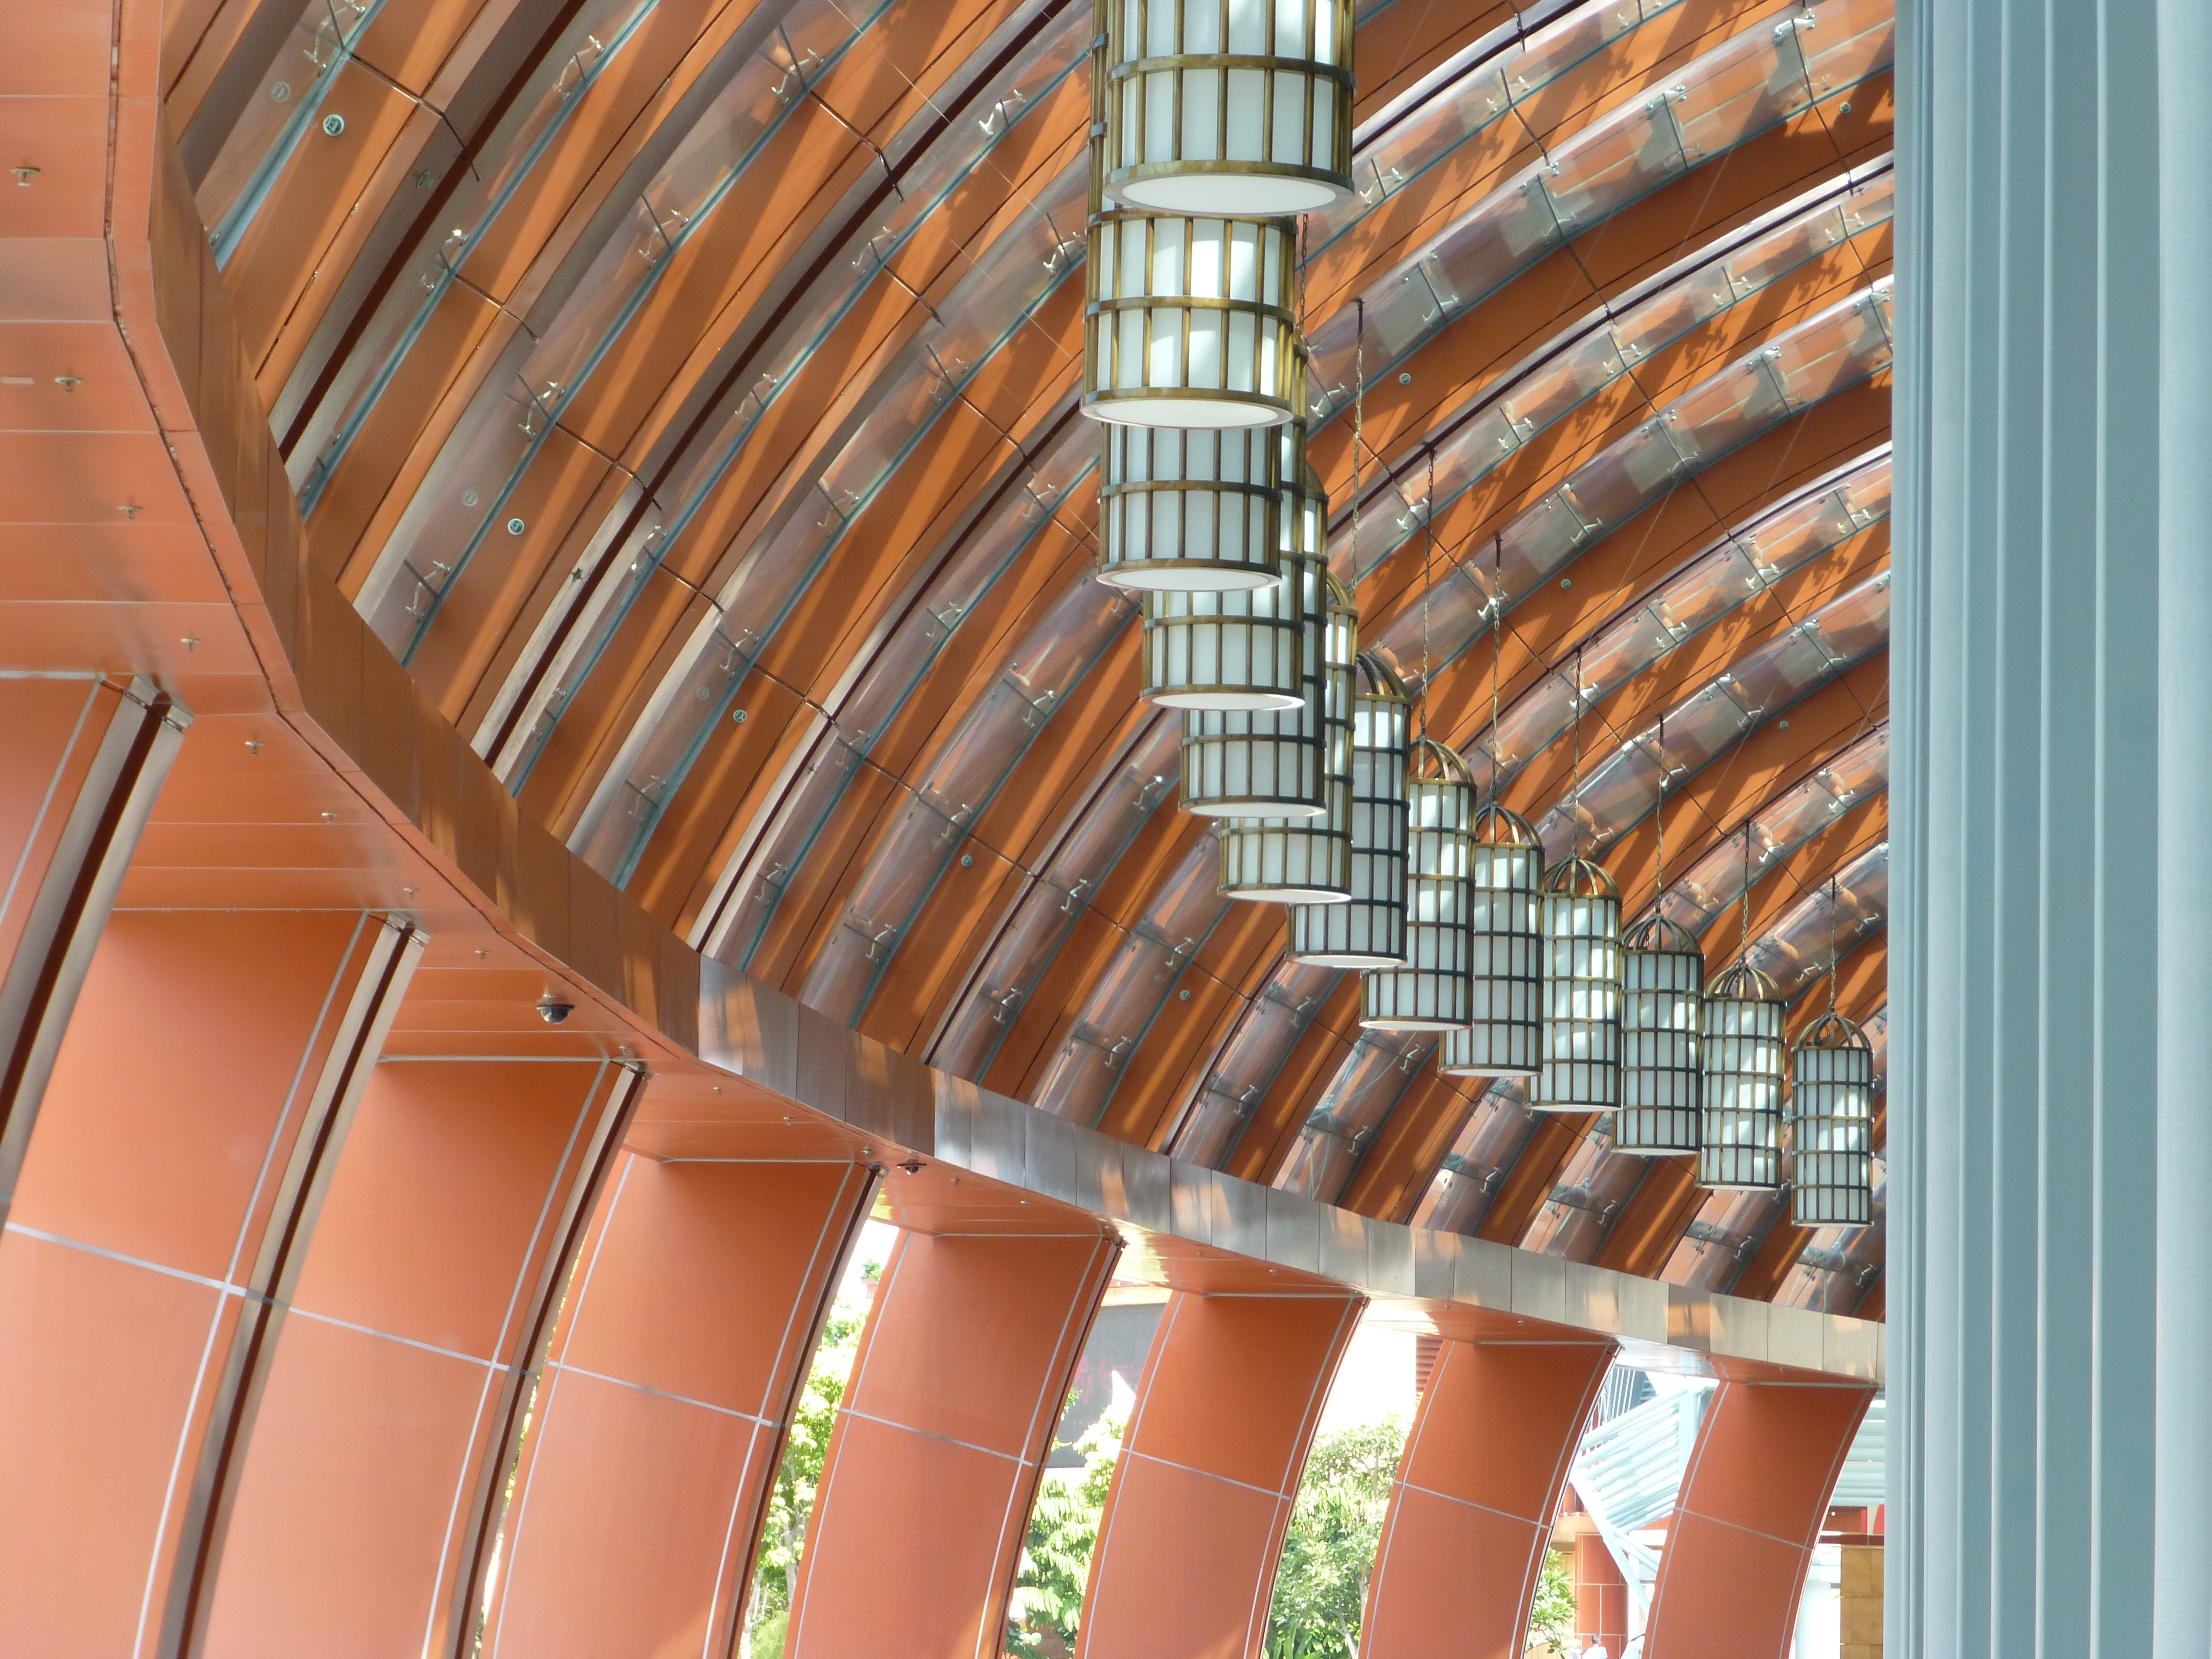
\includegraphics[scale=0.35]
    {figures/jpg/pic04.jpg}
\end{center}
\end{frame}
%-----------------------------------------------------------------------
\section{Lists}
\subsection{Computing with lists}

\begin{frame}[fragile]
\frametitle{Computing with lists}

\begin{itemize}
\item There are two approaches to working with lists:
  \begin{itemize}
  \item Write functions to do what you want, using recursive
    definitions that traverse the list structure.
  \item Write combinations of the standard list processing functions.
  \end{itemize}
\item The second approach is preferred, but the standard
  list processing functions do need to be defined, and those
  definitions use the first approach (recursive definitions).
\item We'll cover both methods.
\end{itemize}

\end{frame}

%-----------------------------------------------------------------------
\subsection{Recursion on lists}

\begin{frame}[fragile]
\frametitle{Recursion on lists}

\begin{itemize}
\item A list is built from the empty list $[]$ and the function $cons\;::\; a\rightarrow [a] \rightarrow [a] $.
\item Every list must be either
  \begin{itemize}
  \item $[]$  or
  \item $(x : xs)$ for some $x$ (the head of the list) and $xs$ (the
    tail).
  \end{itemize}
where  $(x :xs)$ is an alternative syntax for $cons\,x\, xs$
\item The recursive definition follows the structure of the data:
  \begin{itemize}
  \item Base case of the recursion is $[]$.
  \item Recursion (or induction) case is $(x : xs)$.
  \end{itemize}

\end{itemize}

\end{frame}


%%-----------------------------------------------------------------------
\begin{frame}[fragile]
\frametitle{Recursive definition of length}

\begin{verbatim}
# length :: [a] -> Int
length [] = 0                  # the base case
length (x:xs) = 1 + length xs  # recursion case
\end{verbatim}

\end{frame}

%-----------------------------------------------------------------------
\subsection{filter}
\begin{frame}[fragile]
\frametitle{$filter$}

\begin{itemize}
\item filter is given a \emph{predicate} (a function that gives a
  Boolean result) and a list, and returns a list of the elements
  that satisfy the predicate.
\end{itemize}

\begin{verbatim}
filter :: (a->Bool) -> [a] -> [a]
\end{verbatim}

Filtering is useful for the ``generate and test'' programming
paradigm.

\begin{verbatim}
filter (<5) [3,9,2,12,6,4] -- > [3,2,4]
\end{verbatim}

\end{frame}

%-----------------------------------------------------------------------
\begin{frame}[fragile]
\frametitle{Recursive definition of $filter$}

\begin{verbatim}
filter :: (a -> Bool) -> [a] -> [a]
filter pred []    = []
filter pred (x:xs)
  | pred x         = x : filter pred xs
  | otherwise      = filter pred xs
\end{verbatim}

\end{frame}

%-----------------------------------------------------------------------
\subsection{Computations over lists}
\begin{frame}[fragile]
\frametitle{Computations over lists}

\begin{itemize}
\item Many computatations that would be for/while loops in an
  imperative language are naturally expressed as list computations
  in a functional language.
\item There are some common cases:
  \begin{itemize}
  \item Perform a computation on each element of a list: $map$
  \item Iterate over a list, from left to right: $foldl$
  \item Iterate over a list, from right to left: $foldr$
  \end{itemize}
\item It's good practice to use these three functions when
  applicable
\item And there are some related functions that we'll see later
\end{itemize}

\end{frame}

%-----------------------------------------------------------------------
%\subsection{Function composition}
\begin{frame}[fragile]
\frametitle{Function composition}

\begin{itemize}
\item We can express a large compution by ``chaining together'' a
  sequence of functions that perform smaller computations
  \begin{enumerate}
  \item Start with an argument of type $a$
  \item Apply a function $g :: a->b$ to it, getting an intermediate
    result of type $b$
  \item Then apply a function  $f :: b->c$ to the intermediate
    result, getting the final result of type $c$
  \end{enumerate}
\item The entire computation (first $g$, then $f$) is written as $f
  \circ g$.
\item This is traditional mathematical notation; just remember that
  in $f \circ g$, the functions are used in right to left order.
  \item Haskell uses \texttt{.} as the function composition operator
\end{itemize}

\begin{verbatim}
 (.) :: (b->c) -> (a->b) -> a -> c
(f . g) x = f (g x)
\end{verbatim}

\end{frame}

%-----------------------------------------------------------------------
\subsection{map}
\begin{frame}[fragile]
\frametitle{$map$}

\begin{itemize}
\item map applies a function to every element of a list
\end{itemize}


\begin{verbatim}
map f [x0,x1,x2] -- > [f x0, f x1, f x2]
\end{verbatim}

\end{frame}

%-----------------------------------------------------------------------
\begin{frame}[fragile]
\frametitle{Composition of maps}

\begin{itemize}
\item \emph{map} is one of the most commonly used tools in your functional
  toolkit
\item A common style is to define a set of simple computations
  using map, and to compose them.
\end{itemize}

\begin{theorem}
map f (map g xs) = map (f $\circ$ g) xs
\end{theorem}

This theorem is frequently used, in both directions.

\end{frame}

%-----------------------------------------------------------------------

\begin{frame}[fragile]
\frametitle{Recursive definition of map}

\begin{verbatim}
map :: (a -> b) -> [a] -> [b]
map _ []     = []
map f (x:xs) = f x : map f xs
\end{verbatim}

\end{frame}

%-----------------------------------------------------------------------
\subsection{foldl}
\begin{frame}
\frametitle{Folding a list}

\begin{itemize}
\item An iteration over a list to produce a singleton value is
  called a \emph{fold}
\item By convention, we will have a list with elements of type $b$,
  and the singleton value will have type $a$
\item There are several variations: folding from the left, folding
  from the right, several variations having to do with
  ``initialisation'', and some more advanced variations.
\item Folds may look tricky at first, but they are extremely
  powerful, and they are used a lot!  And they aren't actually very
  complicated.
\end{itemize}

\end{frame}

%-----------------------------------------------------------------------
\begin{frame}[fragile]
\frametitle{\emph{foldl}}

\begin{itemize}
\item foldl is \emph{fold from the left}
\item Think of it as an iteration across a list, going left to
  right.
\item A typical application is $foldl\, f\, a\, xs$
\item The $xs :: [b]$ argument is a list
\item A useful intuition: think of the $a :: a$ argument is an
  ``accumulator''.
\item The function takes the current value of the accumulator and a
  list element, and gives the new value of the accumulator.
\end{itemize}

\begin{verbatim}
foldl :: (a->b->a) -> a -> [b] -> a
\end{verbatim}

\end{frame}

%-----------------------------------------------------------------------
\begin{frame}
\frametitle{Examples of foldl with function notation}

\begin{eqnarray*}
\mathtt{foldl\,f\,a\,[]} & \rightsquigarrow & a\\
\mathtt{foldl\,f\,a\,[x0]} & \rightsquigarrow  & f\,a\,x0\\
\mathtt{foldl\,f\,a\,[x0,x1]} & \rightsquigarrow  & f\,(f\,a\,x0)\,x1\\
\mathtt{foldl\,f\,a\,[x0,x1,x2]} & \rightsquigarrow  & f\,(f\,(f\,a\,x0)\,x1)\, x2
\end{eqnarray*}

\end{frame}

%-----------------------------------------------------------------------
\begin{frame}[fragile]
\frametitle{Examples of foldl with infix notation}

In this example, + denotes an arbitrary operator for f; it isn't
supposed to mean specifically addition.

\begin{verbatim}
foldl (+) a []          -- > a
foldl (+) a [x0]        -- > a + x0
foldl (+) a [x0,x1]     -- > (a + x0) + x1
foldl (+) a [x0,x1,x2]  -- > ((a + x0) + x1) + x2
\end{verbatim}

\end{frame}

%-----------------------------------------------------------------------
\begin{frame}[fragile]
\frametitle{Recursive definition of foldl}

\begin{verbatim}
foldl        :: (b -> a -> b) -> b -> [a] -> b
foldl f z0 xs0 = lgo z0 xs0
             where
                lgo z []     =  z
                lgo z (x:xs) = lgo (f z x) xs
\end{verbatim}

\end{frame}

%-----------------------------------------------------------------------
\subsection{foldr}

\begin{frame}[fragile]
\frametitle{$foldr$}
\begin{itemize}
\item Similar to $foldl$, but it works from right to left
\end{itemize}

\begin{verbatim}
foldr :: (a -> b -> b) -> b -> [a] -> b
\end{verbatim}

\end{frame}

%-----------------------------------------------------------------------
\begin{frame}[fragile]
\frametitle{Examples of foldr with function notation}

\begin{eqnarray*}
\mathtt{foldr\,f\, a\, []            } & \rightsquigarrow & a\\
\mathtt{foldr\, f\, a\, [x0]          } & \rightsquigarrow & f\, x0\, a\\
\mathtt{foldr\, f\, a\, [x0,x1]       } & \rightsquigarrow &  f\, x0\, (f\, x1\, a)\\
\mathtt{foldr\, f\, a\, [x0,x1,x2]   } & \rightsquigarrow & f\, x0\, (f\, x1\, (f\, x2\, a))
\end{eqnarray*}

\end{frame}

%-----------------------------------------------------------------------
\begin{frame}[fragile]
\frametitle{Examples of foldr with operator notation}

\begin{verbatim}
foldr (+) a []          -- > a
foldr (+) a [x0]        -- > x0 + a
foldr (+) a [x0,x1]     -- > x0 + (x1 + a)
foldr (+) a [x0,x1,x2]  -- > x0 + (x1 + (x2 + a))
\end{verbatim}

\end{frame}

%-----------------------------------------------------------------------
\begin{frame}[fragile]
\frametitle{Recursive definition of foldr}

\begin{verbatim}
foldr            :: (a -> b -> b) -> b -> [a] -> b
foldr k z = go
          where
            go []     = z
            go (y:ys) = y `k` go ys
\end{verbatim}

\end{frame}

%-----------------------------------------------------------------------
\begin{frame}[fragile]
\frametitle{Relationship between $foldr$ and list structure}
We have seen that a list \texttt{[x0,x1,x2]} can also be written as

\begin{verbatim}
	x0 :  x1 : x2 : []
\end{verbatim}

Folding $cons$ (:) over a list using the empty list [] as accumulator gives:

\begin{verbatim}
foldr (:)  [] [x0,x1,x2]
  -- > x0 :  x1 : x2 : []
\end{verbatim}

This is identical to constructing the list using (:) and [] !

\end{frame}


%-----------------------------------------------------------------------
\begin{frame}[fragile]
\frametitle{Formalising the relationship}

\begin{theorem}
foldr cons [] xs = xs
\end{theorem}

\end{frame}

%-----------------------------------------------------------------------
\begin{frame}[fragile]
\frametitle{Some applications of folds}

\begin{verbatim}
sum xs = foldr (+) 0 xs
product xs = foldr (*) 1 xs
\end{verbatim}

We can actually ``factor out'' the $xs$ that appears at the right
of each side of the equation, and write:

\begin{verbatim}
sum      = foldr (+) 0
product  = foldr (*) 1
\end{verbatim}

(This is sometimes called ``point free'' style because you're
programming solely with the functions; the data isn't mentioned
directly.)

\end{frame}
%
%%-----------------------------------------------------------------------
%\section{Algebraic data types}
%\begin{frame}[fragile]
%\frametitle{Algebraic data types}

%\begin{itemize}
%\item The fundamental mechanism for defining data structures in
%  Haskell is \emph{algebraic data types}
%  \begin{itemize}
%  \item Don't confuse these with abstract data types.  Haskell has
%    those too, and they are quite different.
%  \item It isn't a good idea to use the acronym ADT---someone is
%    sure to misunderstand you.
%  \end{itemize}
%\end{itemize}

%\end{frame}

%%-----------------------------------------------------------------------
%\begin{frame}[fragile]
%\frametitle{Form of an algebraic data type}

%\begin{itemize}
%\item Define the type with a $data$ declaration
%\item There are one or more alternatives separated by $\mid$
%\item Each alternative starts with a \emph{constructor}, a name
%  that must begin with an upper case letter, followed by zero or
%  more types of the fields
%\item The algebraic data type may be just a monomorphic type
%  (e.g. $Bool$ or $Foo$) or it may be polymorphic (e.g. $Tree a b$).
%\end{itemize}

%\end{frame}

%%-----------------------------------------------------------------------
%\begin{frame}[fragile]
%\frametitle{Bool is just an algebraic data type}

%Bool is defined in the standard libraries:

%\begin{verbatim}
%data Bool = False $ True
%\end{verbatim}

%\end{frame}

%%-----------------------------------------------------------------------
%\begin{frame}[fragile]
%\frametitle{Tuples are algebraic data types with sugar}

%We could define tuples like this:

%\begin{verbatim}
%data Pair a b = Pair a b           -- (a,b)
%data Triple a b c = Triple a b c   -- (a,b,c)
%\end{verbatim}

%That's essentially the way tuples are implemented in Haskell,
%except that there is ``syntactic sugar'' so you can write $(a,b)$
%rather than $Pair a b$.

%\end{frame}

%%-----------------------------------------------------------------------
%\begin{frame}[fragile]
%\frametitle{Trees}

%\begin{itemize}
%\item There are many different kinds of trees, so we really don't
%  want to pick just one form, turn it into a built-in feature of
%  the language, and force programmers to shoe-horn all their own
%  data structures into this form.
%\item Trees are easy to define using algebraic data types
%\item Warning: each constructor name must be unique (within a
%  script file or module)
%\end{itemize}

%\begin{verbatim}
%data BinTreeNum = Leaf Int $ Node BinTreeNum BinTreeNum
%data BinTreeNum = Leaf Int $ Node Int BinTreeNum BinTreeNum

%data BinTree a = Tip $ Node a (BinTree a) (BinTree a)
%\end{verbatim}

%\end{frame}



\end{document}
